\chapter{Reconstruction}

A telescope is only as good as it's ability to identify distinct sources. In the case of a neutrino telescope this translates directly to how well observed events can be reconstructed for the direction of high energy events. IceCube uses several reconstruction methods \cite{icecube} and has several data quality checks it must go through before a result is given any weight. Similarly, ANTARES has had years of work put into the reconstruction software in order to reach the accuracies it can now \cite{antares}. To set the context for reconstructions, we need to first understand the data that is collected and how it appears. 

\section{Geometry of a Single Hit}

At first thought, it may sound simple to try and reproduce the tracks that produce the light one would observe in neutrino detectors, but upon considering the data that is aquired the true complexity is revealed. To see this, we consider first the geometry of a single hit to see what the data would look like. Referring to Figure \ref{fig:ghit}, we consider a muon track that is infinite in length, which is a safe approximation assuming a sufficient energy of the neutrino relative to the size of the detector. Specifically we can parameterize the track with
\begin{equation}
  \vec{u}(t) = \vec{x} + ct\vec{v}\, ,
\end{equation}
where $\vec{x}$ is the vertex, $\vec{v}$ is the direction the muon is travelling in, $t$ is the time parameter, and finally $c$ is the speed of light, which again for sufficiently high energy muons is a good approximation for the speed. Looking at the $i^{\text{th}}$ DOM located at a position $\vec{r_{i}}$, it is easy to see there must be a closest approach position for the track, $\vec{p}_{i}$, and emission point of a photon given there is a direct hit on the DOM, located at $\vec{q}_{i}$. The photon is emitted at a cherenkov angle of $\theta_{c}$, which is as described in equation \ref{fig:cher_angle}. 


\begin{figure}
  \centering
  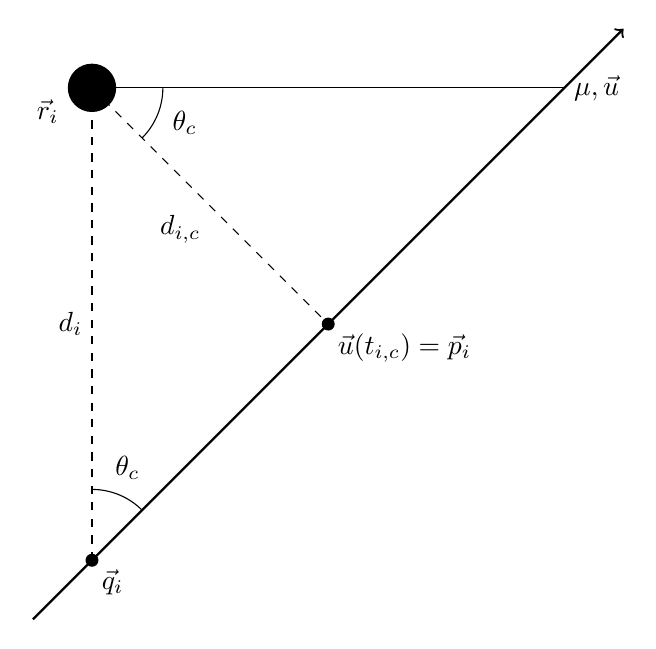
\begin{tikzpicture}[scale=3]
    % Closest point to DOM
    \node [below right] at (0,0) {$\vec{u}(t_{i,c}) = \vec{p}_{i}$};
    \node [below left] at (-0.5, 0.5) {$d_{i,c}$};
    \draw[fill] (0,0) circle [radius=0.025];
    \draw [dashed] (-1,1) -- (0,0);
    % Muon Travel line
    \draw [thick, ->] (-1.25,-1.25) -- (1.25,1.25);
    \node [right] at (1,1) {$\mu, \vec{u}$};
    % Emission point
    \node [below right] at (-1,-1) {$\vec{q}_{i}$};
    \node [above] at (-0.85, -0.7) {$\theta_{c}$};
    \draw[fill] (-1,-1) circle [radius=0.025];
    \draw (-1,-0.7) arc [radius=0.3, start angle=90, end angle=45];
    % DOM
    \node [left] at (-1.1,0.9) {$\vec{r}_{i}$};
    \draw[fill] (-1,1) circle [radius=0.1];
    % Emission Photon
    \node [left] at (-1,0) {$d_{i}$};
    \draw [dashed] (-1,-1) -- (-1,1);
    % Light Wavefront
    \node [right] at (-0.7,0.85) {$\theta_{c}$};
    \draw (-1,1) -- (1,1);
    \draw (-0.7,1) arc [radius=0.3, start angle=0, end angle=-45];
  \end{tikzpicture}
  \caption{Drawing of muon track and Vavilov-Cherenkov Radiation hitting a single DOM.}
  \label{fig:ghit}
\end{figure}



There are several software techniques that need to be applied before a result can be taken seriously, and usually this pipline begins with a simple and quick initial guess fit. 

\section{Linefit}

Any robust reconstruction method requires an initial guess (generally referred to as a seed) in order to be used, but getting this first guess can be non-trivial. Moreover, reconstruction pipelines can be incredibly sensitive to the initial guess and ensuring the quality of this fit is difficult in its own right.

The standard method for a first guess in such situations is the linefit/linear fit. This is a simple track fit that minimizes the $\chi^{2}$ on the observed hits given in an event. 


% Can add charge section (make sure to credit Thomas in statement of originality)
\section{Likelihood}


